
\section{System Co-Design: Smart SSD for Lucene}\label{sec:design}
This section describes the system co-design of the Smart SSD and Lucene.
We first explore the design space in Section~\ref{sec:designSpace} to determine what query processing logic could be cost-effectively offloaded, and then show the co-design architecture of the Smart SSD and Lucene in Section~\ref{sec:sysArch}.

\subsection{Design Space}\label{sec:designSpace}

The overall research question of the co-design is \emph{what query processing logic could be cost-effectively executed by Smart SSDs?} To answer this, we need to understand the opportunities and limitations of Smart SSDs. %(summarized in Table~\ref{tab:SmartSSDProCon}).

\textbf{Opportunities of Smart SSDs}. Executing I/O operations inside Smart SSDs is very fast for the following two reasons. (1) SSDs generally provide several times higher internal bandwidth than the host I/O interface bandwidth~\cite{Do2013QPS,De2013}. In our Smart SSD, the internal bandwidth is around 3.2 GB/s, while the host I/O bandwidth is around 750 MB/s. (2) The I/O latency inside Smart SSDs is very low compared to a regular I/O issued from the host system. A regular I/O operation (from flash chips to the host DRAM) needs to go through the entire thick OS stack, which introduces a lot of overheads such as interrupt, context switch, and file system overhead.
%--file system, interrupt, context switch between the kernel space and the user space--which is collectively called OS software overhead.
The OS software overhead becomes a crucial factor in SSDs due to their fast I/O (but it can be negligible in HDDs as their slow I/O is a dominant factor)~\cite{Caulfield2010}. However, an I/O operation inside SSDs (from flash chips to the DRAM inside SSD) is free from the OS software overhead. Thus, it is very profitable to execute \emph{I/O-intensive} operations inside SSDs to leverage their high internal bandwidth and low I/O latency. %Smart SSDs can reduce the I/O time significantly.

\textbf{Limitations of Smart SSDs}. Smart SSDs also have some limitations. (1) Generally, Smart SSDs employ low-frequency processors (typically ARM series) to save energy and manufacturing cost. As a result, computing capability is several times lower than host CPUs (e.g., Intel processor)~\cite{Do2013QPS,De2013}; (2) The Smart SSD also has a DRAM inside. Accessing the device DRAM is slower than the host DRAM because typical SSD controllers do not adopt caches\footnote{\small Although there is SRAM inside SSDs, it is not generally used for data caching.} (e.g., L1/L2 caches). Therefore, it is not desirable to execute \emph{CPU-intensive} and \emph{memory-intensive} operations inside SSDs. %That means, Smart SSDs will increase the CPU time.

Smart SSDs can reduce the I/O time at the expense of the increasing CPU time so that a system with I/O time bottleneck can notably benefit from Smart SSDs. As an example, the Lucene system running on regular SSDs has an I/O time bottleneck, see Figure~\ref{fig:timeBreakDownRegularSSD} (please refer to Section~\ref{sec:expSetup} for more experimental settings). We observe the I/O time of a typical real-world query is 54.8 ms while its CPU time is 8 ms. Thus, offloading this query to Smart SSDs can significantly reduce the I/O time. Figure~\ref{fig:timeBreakDownRegSmart} in Section~\ref{sec:expResults} supports this claim.  If we offload steps S3 and S4 to Smart SSDs, the I/O time reduces to 14.5 ms while the CPU time increases to 16.6 ms. Overall, Smart SSDs can reduce the total time by a factor of 2.

%Hence, for any system that could potentially benefit from Smart SSDs, should be bottlenecked on the I/O time (if executed on regular SSDs). Otherwise, Smart SSDs could not reduce the query latency.


%However, for Lucene system running on regular SSD, the I/O time is still a bottleneck, see Figure~\ref{fig:timeBreakDownRegularSSD} (refer to Section~\ref{sec:expResults} for more experimental settings). We see that, the I/O time is 54.8 ms while the CPU time is 8 ms. Thus, offloading queries to Smart SSDs can reduce the I/O time significantly. In Section~\ref{sec:expResults} (Figure~\ref{fig:timeBreakDownRegSmart}), we show that, for the same query on Smart SSDs, if we offload step S3 and S4 to Smart SSDs, the I/O time can be reduce to 14.5 ms while the CPU time is increased to 16.6 ms. Thus, Smart SSDs can reduce the total time by a factor of 2.

\begin{figure}[htbp]
%\vspace{-5mm}
	\centering
		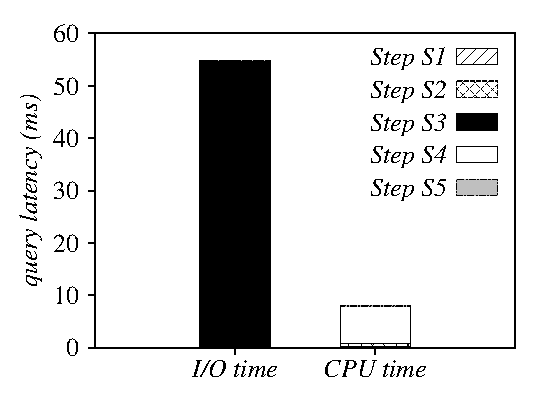
\includegraphics[width=0.55\columnwidth]{figures/timeBreakDownRegularSSD.eps}
	\caption{Time breakdown of executing a typical real-world query by Lucene system running on regular SSDs}
	\label{fig:timeBreakDownRegularSSD}
\end{figure}




%\begin{table}[htbp]
%\centering\small
%\begin{tabular}{l|l}\hline\hline
%\textbf{Opportunities}    & \textbf{Limitations}\\\hline
%P1. High internal bandwidth & C1. CPU is slow \\\hline
%P2. Low I/O latency & C2. DRAM access is slow\\\hline\hline
%\end{tabular}
%\caption{Pros and cons of Smart SSD}\label{tab:SmartSSDProCon}
%\end{table}



Based on this observation, we next analyze what query processing steps in Lucene (namely, step S1 -- S5 in Figure~\ref{fig:searchEngineArch}) could be executed inside SSDs to reduce both query latency and power consumption. We make a rough analysis first and then evaluate them by experiments thoroughly.

\textbf{Step S1: Parse query}. Parsing a query involves a number of CPU-intensive steps such as tokenization, stemming, and lemmatization~\cite{M08}. Thus, it is not profitable to offload this step S1.% to Smart SSDs.

\textbf{Step S2: Get metadata}. The metadata is essentially a key-value pair. The key is a query term and the value is the basic information about the on-disk inverted list of the term.  In Lucene, it contains (1) the offset where the list is stored on disk, (2) the length (in bytes) of the list, and (3) the number of entries in the list. The metadata is stored in a dictionary file. There is a Btree-like data structure built for the dictionary file. Since it takes very few (usually 1 $\sim$ 2) I/O operations to obtain the metadata~\cite{M08}, we do not offload this step.

\textbf{Step S3: Get inverted lists}. Each inverted list contains a list of documents containing the same term.
Since Lucene stores all the inverted lists on a disk and does not adopt caching to save memory\footnote{\small Even though other search engines may cache inverted lists in the host memory, it may not solve the I/O problem. (1) The cache hit ratio is low even for big memories, typically 30\% to 60\% due to the cache invalidation caused by inverted index update~\cite{Barroso2003WSP}. (2) Big DRAM in the host side consumes too much energy because of the periodic memory refreshment~\cite{Hennessy2006}.}, upon receiving a query, it reads the inverted lists from the disk to the host memory, which is I/O-intensive.
As is shown in Figure~\ref{fig:timeBreakDownRegularSSD}, the step S3 takes 87\% of the time if Lucene runs on regular SSDs. Therefore, it is desirable to offload this step to Smart SSDs.


\textbf{Step S4: Execute list operations}. The main reason of loading inverted lists to the host memory is to efficiently execute list operations such as intersection. Thus, both steps S4 and S3 should be offloaded to Smart SSDs. This raises another question: what operation(s) could potentially benefit from Smart SSDs. In Lucene, there are three basic operations commonly used: list \textsf{intersection}, \textsf{union}, and \textsf{difference}. They are also widely adopted in many commercial search engines (e.g., Google advanced search\footnote{\small\url{http://www.google.com/advanced_search}}). We investigate each operation and set up a simple principle that the output size should be smaller than its input size. Otherwise, Smart SSDs cannot save any data movement. Let $A$ and $B$ be two inverted lists, and we assume $A$ is shorter than $B$ to capture the real case of skewed lists.
\begin{itemize}%[noitemsep, topsep=2pt]
  \item \textsf{Intersection}: The result size of the intersection is usually much smaller compared to each inverted list, i.e., $|A\cap B| \ll |A| + |B|$. E.g., in Bing search, for 76\% of the queries, the intersection result size is two orders of magnitude smaller than the shortest inverted list involved~\cite{Ding2011}. Similar results are observed in our real dataset. Thus, executing intersection inside SSDs may be a smart choice as it can save a lot of host I/O interface bandwidth.

  \item \textsf{Union}: The union result size can be similar to the total size of the inverted lists. That is because $|A\cup B| = |A| + |B| - |A\cap B|$, while typically $|A\cap B| \ll |A| + |B|$, then $|A\cup B| \approx |A| + |B|$. Unless $|A\cap B|$ is similar to $|A| + |B|$. An extreme case is $A = B$, then $|A\cup B| = |A| = |B|$, meaning that we can save 50\% of data transfer. However, in general, it is not cost-effective to offload \textsf{union} to Smart SSDs.

  \item \textsf{Difference}: It is used to find all the documents in one list but not in the other list. Since this operation is ordering-sensitive, we consider two cases: $(A - B)$ and $(B - A)$. For the former case, $|A - B| = |A| - |A\cap B| < |A| \ll |A| + |B|$. That is, sending the results of $(A - B)$ saves a lot of data transfer if executed in Smart SSDs. On the other hand, the latter case may not save much data transfer because $|B - A| = |B| - |A\cap B| \approx |B| \approx |B| + |A|$. Consequently, we still consider the \textsf{difference} as a possible candidate for query offloading.
\end{itemize}

\textbf{Step S5: Compute similarity and rank}. After the aforementioned list operations are completed, we can get a list of qualified documents\footnote{\small Lucene assumes the results are small enough to fit into main memory, thus, no any I/O involved.}. %Lucene assumes the results are small enough to fit into main memory.
This step applies a ranking model to the qualified documents in order to determine the similarities between the query and these documents. This is because users are more interested in the most relevant documents. This step is CPU-intensive so that it may not be a good candidate to offload to Smart SSDs. However, it is beneficial when the result size is very large because after step S5, only the top ranked results are returned. This can save a lot of I/Os. From the design point of view, we can consider two options: (1) do not offload step S5. In this case, step S5 is executed at the host side; (2) offload this step. In this case, step S5 is executed by Smart SSDs.


\begin{table}[htbp]\small
\centering
\begin{tabular}{l|c|c}\hline\hline
&Non-Ranked & Ranked \\\hline
\textsf{Intersection} & \ding{51} & \ding{51} \\\hline
\textsf{Union} &\ding{55}  & \ding{51}\\\hline
\textsf{Difference} & \ding{51}& \ding{51}\\\hline\hline
\end{tabular}
\caption{Design space}\label{tab:designSpace}
\end{table}
In summary, we consider offloading five query operations that could potentially benefit from Smart SSDs: \textsf{intersection}, \textsf{ranked intersection}, \textsf{ranked union}, \textsf{difference}, and \textsf{ranked difference} (see Table~\ref{tab:designSpace}). The offloading of non-ranked operations means that only steps S3 and S4 will be executed inside SSDs while step S5 is executed at the host side. The offloading of ranked operations means that all steps S3, S4, and S5 will be executed inside SSDs. In either case, steps S1 and S2 are executed at the host side.

%We note that Lucene may not embrace all state-of-the-art query processing techniques. E.g., step S4 and S5 could be algorithmically combined for early termination~\cite{Broder2003EQE,Fagin2001}.

\subsection{System Co-Design Architecture}\label{sec:sysArch}

\begin{figure}[htbp]
  \centering
  \begin{tabular}{ccc}
 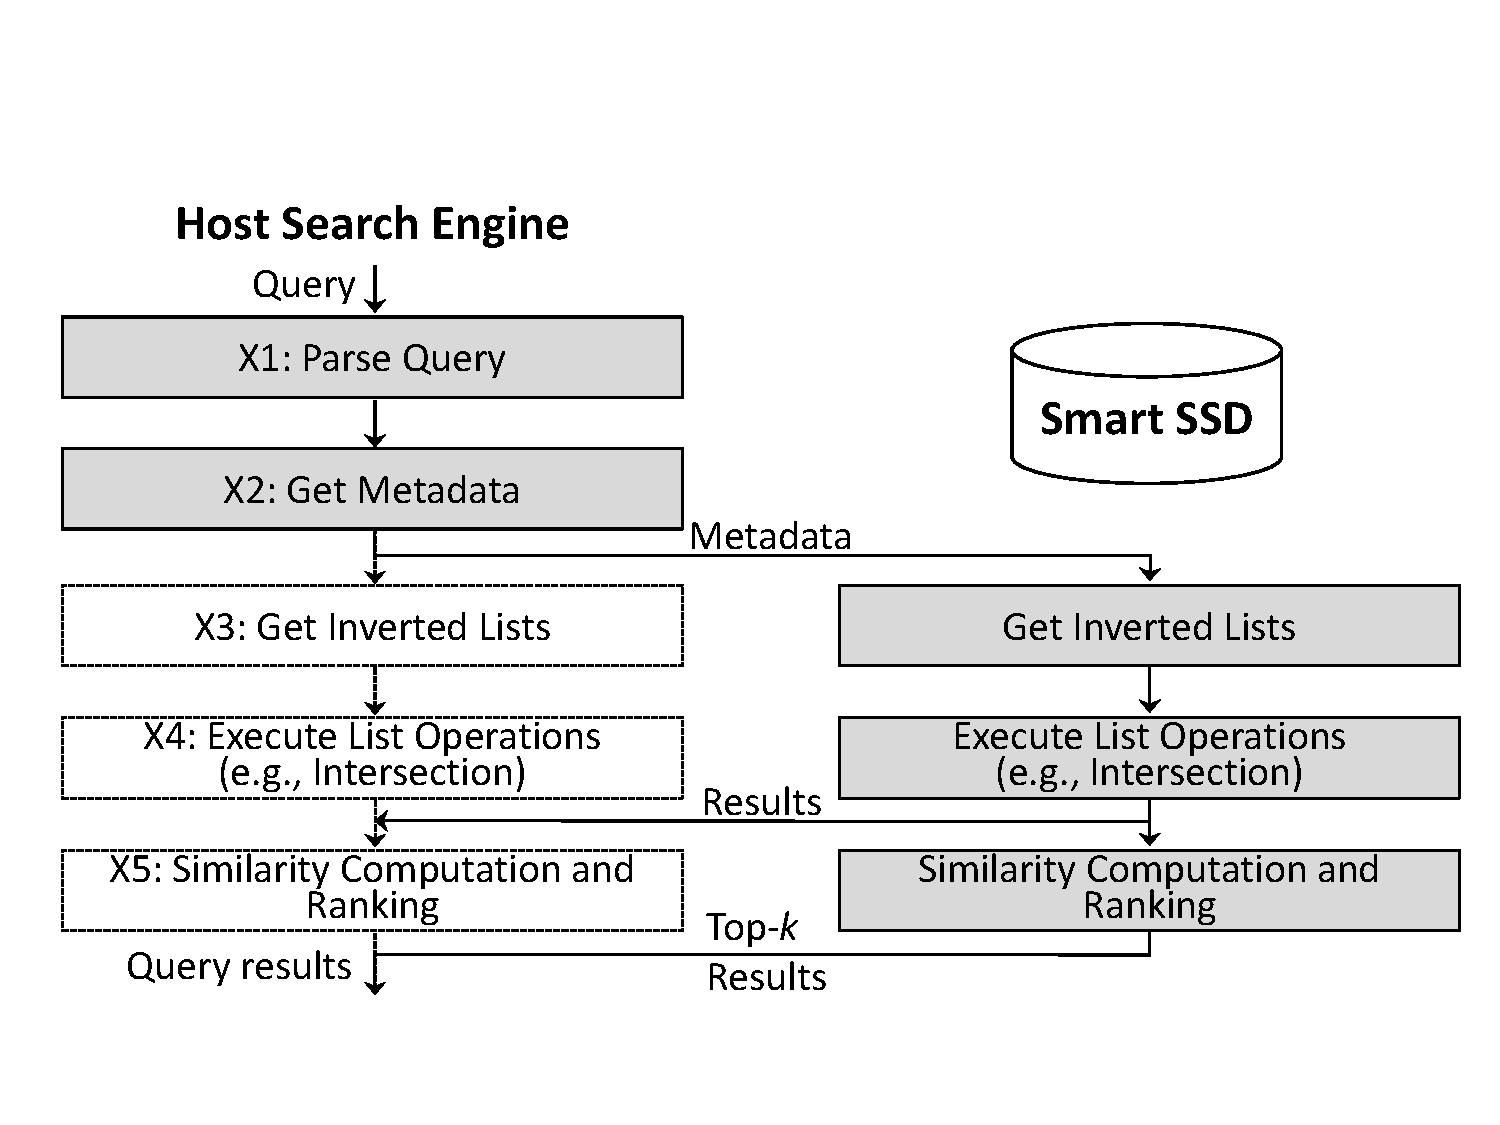
\includegraphics[width=1.0\columnwidth]{figures/SmartSSDLucene.pdf}
\end{tabular}
  \caption{Co-design architecture of Lucene and Smart SSDs}
  \label{fig:SmartSSDLucene}
 \end{figure}

Figure~\ref{fig:SmartSSDLucene} shows the co-design architecture of Lucene search engine and the Smart SSD. We modified Lucene code following the architecture such that Lucene can interact with the Smart SSD.
%We integrated Smart SSD with Lucene (an open source search engine) following this architecture. Thus, Lucene can directly interact with Smart SSD.

It operates as follows. Assume only the \textsf{intersection} operation is offloaded. The host Lucene is responsible for receiving queries. Upon receiving a query $q(t_1,t_2,...,t_u)$, where each $t_i$ is a query term. Lucene parses the query $q$ to $u$ query terms (Step S1) and gets the metadata for each query term $t_i$ (Step S2). Then, it sends all the metadata information to Smart SSDs via the OPEN API.
The Smart SSD now starts to load the $u$ inverted lists to the device memory (DRAM) using the metadata. The device DRAM is generally of several hundred MBs, which is big enough to store the inverted lists of a typical query.
When all the $u$ inverted lists are loaded to the device DRAM, the Smart SSD executes list intersection. Once it is done, the results will be put to an output buffer and ready to be returned to the host side.
The host Lucene keeps monitoring the status of Smart SSDs in a heart-beat manner via the GET API. We set the polling interval to be 1 ms. Once the host Lucene receives the intersection results, it executes step S5 to complete the query, and returns the top ranked results to end users. If the ranked operation is offloaded, Smart SSDs will also take care of step S5.
